% fig/fig_architecture.tex -- MoRE block diagram (pure TikZ, compact layout).
% Needs only \usepackage{tikz} in the preamble (no \usetikzlibrary).
% In sections/02_method.tex replace the old figure* block by: % fig/fig_architecture.tex -- MoRE block diagram (pure TikZ, compact layout).
% Needs only \usepackage{tikz} in the preamble (no \usetikzlibrary).
% In sections/02_method.tex replace the old figure* block by: % fig/fig_architecture.tex -- MoRE block diagram (pure TikZ, compact layout).
% Needs only \usepackage{tikz} in the preamble (no \usetikzlibrary).
% In sections/02_method.tex replace the old figure* block by: % fig/fig_architecture.tex -- MoRE block diagram (pure TikZ, compact layout).
% Needs only \usepackage{tikz} in the preamble (no \usetikzlibrary).
% In sections/02_method.tex replace the old figure* block by: \input{fig/fig_architecture}
\begin{figure}[t]
\centering
\resizebox{\textwidth}{!}{%
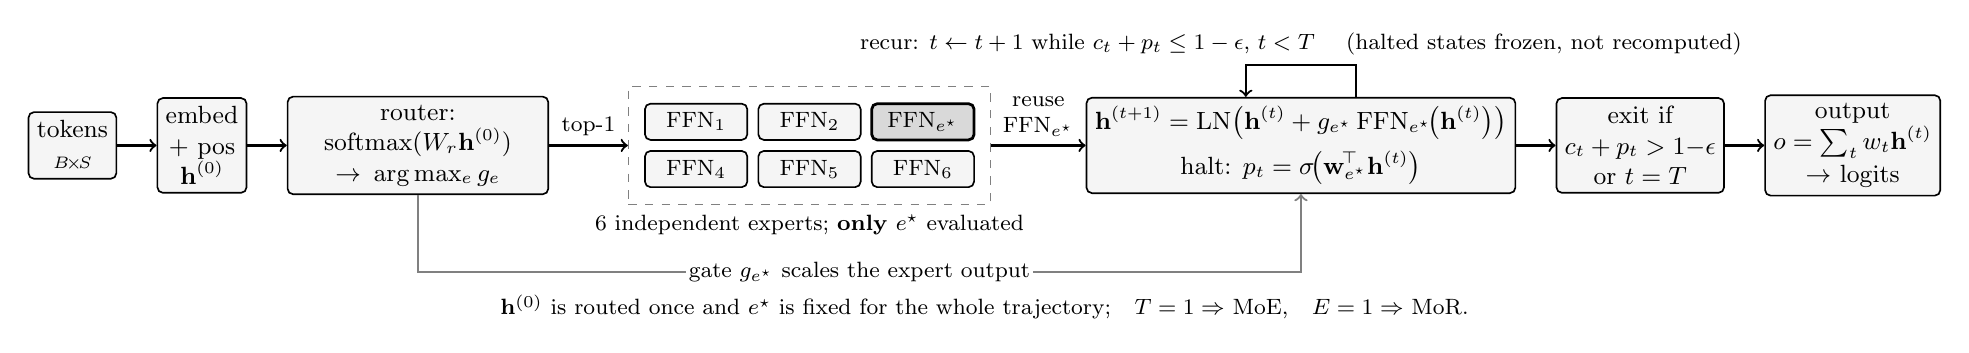
\begin{tikzpicture}[font=\small]
  \tikzset{
    box/.style = {draw, rounded corners=2pt, align=center, inner sep=3pt,
                  minimum height=7mm, line width=0.6pt},
    st/.style  = {box, fill=black!4},
    ex/.style  = {box, fill=black!4, minimum width=13mm, minimum height=4.6mm,
                  inner sep=1.5pt, font=\footnotesize},
    sel/.style = {box, fill=black!15, minimum width=13mm, minimum height=4.6mm,
                  inner sep=1.5pt, font=\footnotesize, line width=1.0pt},
    nb/.style  = {font=\footnotesize, align=center, inner sep=2pt},
    ar/.style  = {->, thick}
  }

  % ---- main row (each node is placed relative to its left neighbour) ----
  \node[st] (tok) at (0,0) {tokens\\ $\scriptstyle B\!\times\!S$};
  \node[st, anchor=west] (emb) at ([xshift=5mm]tok.east) {embed\\ $+$ pos\\ $\mathbf{h}^{(0)}$};
  \node[st, anchor=west, text width=31mm] (rtr) at ([xshift=5mm]emb.east)
       {router:\\ $\mathrm{softmax}(W_r\mathbf{h}^{(0)})$\\ $\to \arg\max_e g_e$};

  % expert bank: 2 x 3 grid, dashed frame
  \node[draw, dashed, gray, anchor=west, minimum width=46mm, minimum height=15mm]
       (bank) at ([xshift=10mm]rtr.east) {};
  \node[ex]  (e1) at ([xshift=-14.4mm,yshift= 3mm]bank.center) {FFN$_{1}$};
  \node[ex]  (e2) at ([xshift=  0mm,  yshift= 3mm]bank.center) {FFN$_{2}$};
  \node[sel] (e3) at ([xshift= 14.4mm,yshift= 3mm]bank.center) {FFN$_{e^\star}$};
  \node[ex]  (e4) at ([xshift=-14.4mm,yshift=-3mm]bank.center) {FFN$_{4}$};
  \node[ex]  (e5) at ([xshift=  0mm,  yshift=-3mm]bank.center) {FFN$_{5}$};
  \node[ex]  (e6) at ([xshift= 14.4mm,yshift=-3mm]bank.center) {FFN$_{6}$};
  \node[nb, anchor=north] at ([yshift=-0.5mm]bank.south)
       {6 independent experts; \textbf{only} $e^\star$ evaluated};

  % tied recursion block (Eq. 1 + Eq. 2)
  \node[st, anchor=west, minimum width=42mm] (rec) at ([xshift=12mm]bank.east)
       {$\mathbf{h}^{(t+1)}=\mathrm{LN}\!\left(
          \mathbf{h}^{(t)} + g_{e^\star}\,\mathrm{FFN}_{e^\star}\!\big(\mathbf{h}^{(t)}\big)
        \right)$\\[3pt]
        halt: $p_t=\sigma\!\big(\mathbf{w}_{e^\star}^{\!\top}\mathbf{h}^{(t)}\big)$};

  % exit decision (Eq. 3) and output
  \node[st, anchor=west] (exit) at ([xshift=5mm]rec.east)
       {exit if\\ $c_t+p_t>1{-}\epsilon$\\ or $t=T$};
  \node[st, anchor=west] (out) at ([xshift=5mm]exit.east)
       {output\\ $o=\sum_t w_t\mathbf{h}^{(t)}$\\[1pt] $\to$ logits};

  % ---- main-path arrows ----
  \draw[ar] (tok) -- (emb);
  \draw[ar] (emb) -- (rtr);
  \draw[ar] (rtr.east) -- (bank.west) node[midway, above=1pt, nb] {top-1};
  \draw[ar] (bank.east) -- (rec.west) node[midway, above=1pt, nb, align=center]
        {reuse\\ $\mathrm{FFN}_{e^\star}$};
  \draw[ar] (rec) -- (exit);
  \draw[ar] (exit) -- (out);

  % gate g_{e*} scales the expert output (router -> recursion block)
  \coordinate (gA) at ([yshift=-8.5mm]rtr.south |- bank.south);
  \coordinate (gB) at (rec.south |- gA);
  \draw[ar, gray] (rtr.south) -- (gA) -- (gB) -- (rec.south);
  \path (gA) -- (gB) node[midway, nb, fill=white, inner sep=1pt] {gate $g_{e^\star}$ scales the expert output};

  % recursion self-loop
  \draw[ar] ([xshift=7mm]rec.north) -- ([xshift=7mm,yshift=4mm]rec.north)
        -- ([xshift=-7mm,yshift=4mm]rec.north) -- ([xshift=-7mm]rec.north);
  \node[nb, anchor=south] at ([yshift=4.5mm]rec.north)
       {recur: $t \leftarrow t+1$ while $c_t+p_t\le 1-\epsilon$, $t<T$
        \quad(halted states frozen, not recomputed)};

  % bottom note
  \node[nb, anchor=north] at ([yshift=-0.5mm]current bounding box.south)
       {$\mathbf{h}^{(0)}$ is routed once and $e^\star$ is fixed for the whole
        trajectory;\quad $T=1\Rightarrow$ MoE,\quad $E=1\Rightarrow$ MoR.};
\end{tikzpicture}}
\caption{The MoRE block, drawn in TikZ. A token is routed \emph{once} from its
post-embedding state to one of $E$ independent expert FFNs, and \emph{that
expert's} weights---never another's---are reused for an adaptive number of
recursion steps under ACT halting. Only the selected expert is evaluated, and
its output is scaled by the gate $g_{e^\star}$. Setting $T=1$ recovers MoE
exactly and setting $E=1$ recovers MoR; the input representation is bit-identical
in all three cases, and all three are configurations of one engine.}
\label{fig:architecture}
\end{figure}

\begin{figure}[t]
\centering
\resizebox{\textwidth}{!}{%
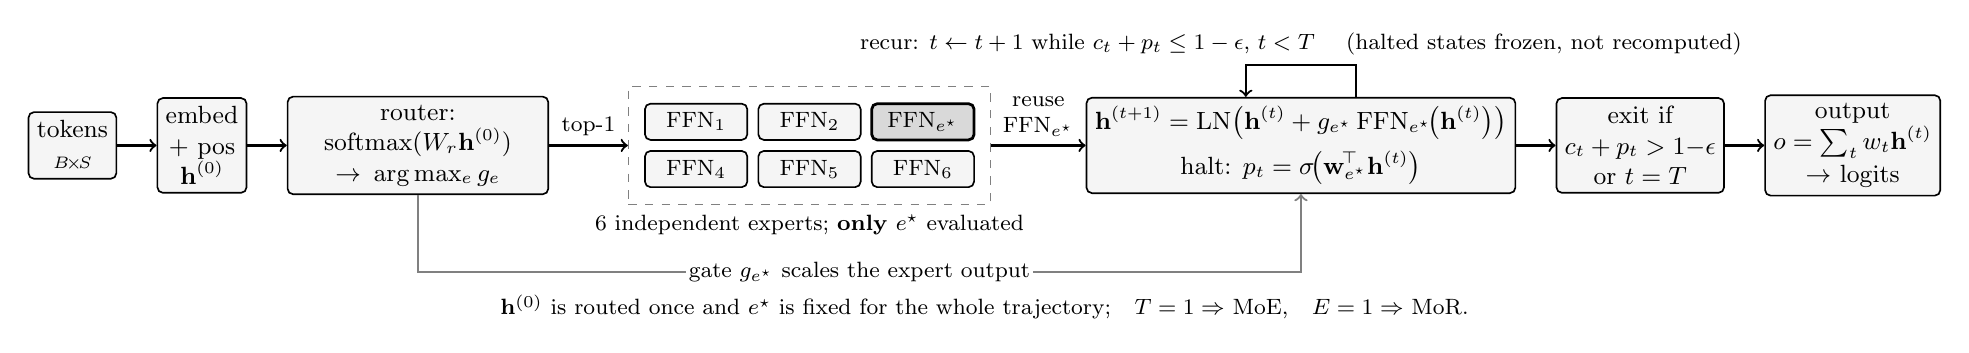
\begin{tikzpicture}[font=\small]
  \tikzset{
    box/.style = {draw, rounded corners=2pt, align=center, inner sep=3pt,
                  minimum height=7mm, line width=0.6pt},
    st/.style  = {box, fill=black!4},
    ex/.style  = {box, fill=black!4, minimum width=13mm, minimum height=4.6mm,
                  inner sep=1.5pt, font=\footnotesize},
    sel/.style = {box, fill=black!15, minimum width=13mm, minimum height=4.6mm,
                  inner sep=1.5pt, font=\footnotesize, line width=1.0pt},
    nb/.style  = {font=\footnotesize, align=center, inner sep=2pt},
    ar/.style  = {->, thick}
  }

  % ---- main row (each node is placed relative to its left neighbour) ----
  \node[st] (tok) at (0,0) {tokens\\ $\scriptstyle B\!\times\!S$};
  \node[st, anchor=west] (emb) at ([xshift=5mm]tok.east) {embed\\ $+$ pos\\ $\mathbf{h}^{(0)}$};
  \node[st, anchor=west, text width=31mm] (rtr) at ([xshift=5mm]emb.east)
       {router:\\ $\mathrm{softmax}(W_r\mathbf{h}^{(0)})$\\ $\to \arg\max_e g_e$};

  % expert bank: 2 x 3 grid, dashed frame
  \node[draw, dashed, gray, anchor=west, minimum width=46mm, minimum height=15mm]
       (bank) at ([xshift=10mm]rtr.east) {};
  \node[ex]  (e1) at ([xshift=-14.4mm,yshift= 3mm]bank.center) {FFN$_{1}$};
  \node[ex]  (e2) at ([xshift=  0mm,  yshift= 3mm]bank.center) {FFN$_{2}$};
  \node[sel] (e3) at ([xshift= 14.4mm,yshift= 3mm]bank.center) {FFN$_{e^\star}$};
  \node[ex]  (e4) at ([xshift=-14.4mm,yshift=-3mm]bank.center) {FFN$_{4}$};
  \node[ex]  (e5) at ([xshift=  0mm,  yshift=-3mm]bank.center) {FFN$_{5}$};
  \node[ex]  (e6) at ([xshift= 14.4mm,yshift=-3mm]bank.center) {FFN$_{6}$};
  \node[nb, anchor=north] at ([yshift=-0.5mm]bank.south)
       {6 independent experts; \textbf{only} $e^\star$ evaluated};

  % tied recursion block (Eq. 1 + Eq. 2)
  \node[st, anchor=west, minimum width=42mm] (rec) at ([xshift=12mm]bank.east)
       {$\mathbf{h}^{(t+1)}=\mathrm{LN}\!\left(
          \mathbf{h}^{(t)} + g_{e^\star}\,\mathrm{FFN}_{e^\star}\!\big(\mathbf{h}^{(t)}\big)
        \right)$\\[3pt]
        halt: $p_t=\sigma\!\big(\mathbf{w}_{e^\star}^{\!\top}\mathbf{h}^{(t)}\big)$};

  % exit decision (Eq. 3) and output
  \node[st, anchor=west] (exit) at ([xshift=5mm]rec.east)
       {exit if\\ $c_t+p_t>1{-}\epsilon$\\ or $t=T$};
  \node[st, anchor=west] (out) at ([xshift=5mm]exit.east)
       {output\\ $o=\sum_t w_t\mathbf{h}^{(t)}$\\[1pt] $\to$ logits};

  % ---- main-path arrows ----
  \draw[ar] (tok) -- (emb);
  \draw[ar] (emb) -- (rtr);
  \draw[ar] (rtr.east) -- (bank.west) node[midway, above=1pt, nb] {top-1};
  \draw[ar] (bank.east) -- (rec.west) node[midway, above=1pt, nb, align=center]
        {reuse\\ $\mathrm{FFN}_{e^\star}$};
  \draw[ar] (rec) -- (exit);
  \draw[ar] (exit) -- (out);

  % gate g_{e*} scales the expert output (router -> recursion block)
  \coordinate (gA) at ([yshift=-8.5mm]rtr.south |- bank.south);
  \coordinate (gB) at (rec.south |- gA);
  \draw[ar, gray] (rtr.south) -- (gA) -- (gB) -- (rec.south);
  \path (gA) -- (gB) node[midway, nb, fill=white, inner sep=1pt] {gate $g_{e^\star}$ scales the expert output};

  % recursion self-loop
  \draw[ar] ([xshift=7mm]rec.north) -- ([xshift=7mm,yshift=4mm]rec.north)
        -- ([xshift=-7mm,yshift=4mm]rec.north) -- ([xshift=-7mm]rec.north);
  \node[nb, anchor=south] at ([yshift=4.5mm]rec.north)
       {recur: $t \leftarrow t+1$ while $c_t+p_t\le 1-\epsilon$, $t<T$
        \quad(halted states frozen, not recomputed)};

  % bottom note
  \node[nb, anchor=north] at ([yshift=-0.5mm]current bounding box.south)
       {$\mathbf{h}^{(0)}$ is routed once and $e^\star$ is fixed for the whole
        trajectory;\quad $T=1\Rightarrow$ MoE,\quad $E=1\Rightarrow$ MoR.};
\end{tikzpicture}}
\caption{The MoRE block, drawn in TikZ. A token is routed \emph{once} from its
post-embedding state to one of $E$ independent expert FFNs, and \emph{that
expert's} weights---never another's---are reused for an adaptive number of
recursion steps under ACT halting. Only the selected expert is evaluated, and
its output is scaled by the gate $g_{e^\star}$. Setting $T=1$ recovers MoE
exactly and setting $E=1$ recovers MoR; the input representation is bit-identical
in all three cases, and all three are configurations of one engine.}
\label{fig:architecture}
\end{figure}

\begin{figure}[t]
\centering
\resizebox{\textwidth}{!}{%
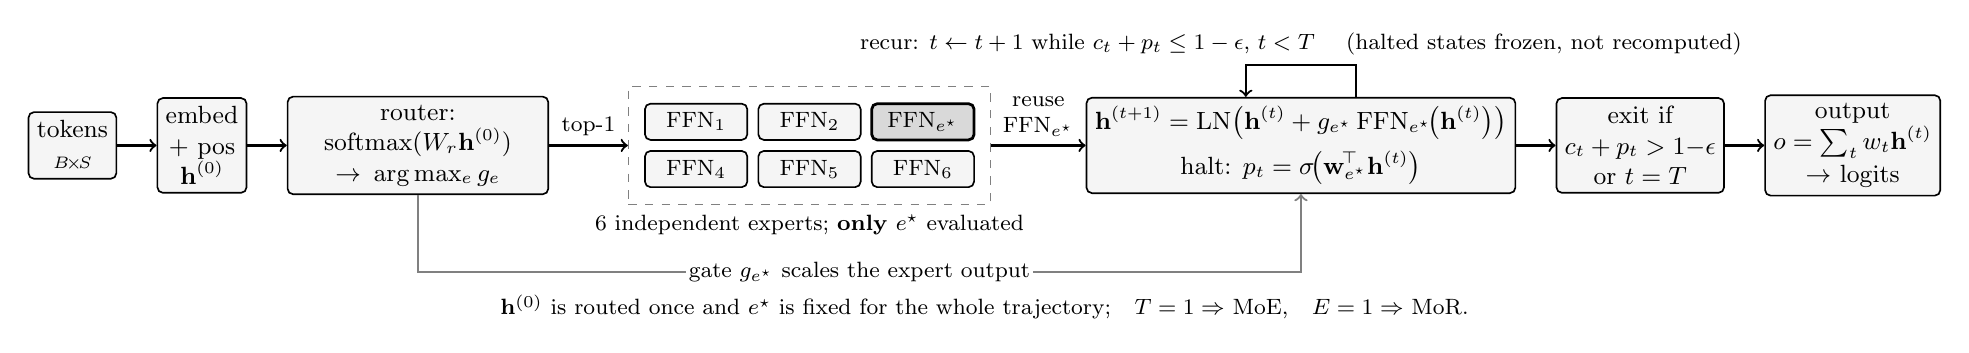
\begin{tikzpicture}[font=\small]
  \tikzset{
    box/.style = {draw, rounded corners=2pt, align=center, inner sep=3pt,
                  minimum height=7mm, line width=0.6pt},
    st/.style  = {box, fill=black!4},
    ex/.style  = {box, fill=black!4, minimum width=13mm, minimum height=4.6mm,
                  inner sep=1.5pt, font=\footnotesize},
    sel/.style = {box, fill=black!15, minimum width=13mm, minimum height=4.6mm,
                  inner sep=1.5pt, font=\footnotesize, line width=1.0pt},
    nb/.style  = {font=\footnotesize, align=center, inner sep=2pt},
    ar/.style  = {->, thick}
  }

  % ---- main row (each node is placed relative to its left neighbour) ----
  \node[st] (tok) at (0,0) {tokens\\ $\scriptstyle B\!\times\!S$};
  \node[st, anchor=west] (emb) at ([xshift=5mm]tok.east) {embed\\ $+$ pos\\ $\mathbf{h}^{(0)}$};
  \node[st, anchor=west, text width=31mm] (rtr) at ([xshift=5mm]emb.east)
       {router:\\ $\mathrm{softmax}(W_r\mathbf{h}^{(0)})$\\ $\to \arg\max_e g_e$};

  % expert bank: 2 x 3 grid, dashed frame
  \node[draw, dashed, gray, anchor=west, minimum width=46mm, minimum height=15mm]
       (bank) at ([xshift=10mm]rtr.east) {};
  \node[ex]  (e1) at ([xshift=-14.4mm,yshift= 3mm]bank.center) {FFN$_{1}$};
  \node[ex]  (e2) at ([xshift=  0mm,  yshift= 3mm]bank.center) {FFN$_{2}$};
  \node[sel] (e3) at ([xshift= 14.4mm,yshift= 3mm]bank.center) {FFN$_{e^\star}$};
  \node[ex]  (e4) at ([xshift=-14.4mm,yshift=-3mm]bank.center) {FFN$_{4}$};
  \node[ex]  (e5) at ([xshift=  0mm,  yshift=-3mm]bank.center) {FFN$_{5}$};
  \node[ex]  (e6) at ([xshift= 14.4mm,yshift=-3mm]bank.center) {FFN$_{6}$};
  \node[nb, anchor=north] at ([yshift=-0.5mm]bank.south)
       {6 independent experts; \textbf{only} $e^\star$ evaluated};

  % tied recursion block (Eq. 1 + Eq. 2)
  \node[st, anchor=west, minimum width=42mm] (rec) at ([xshift=12mm]bank.east)
       {$\mathbf{h}^{(t+1)}=\mathrm{LN}\!\left(
          \mathbf{h}^{(t)} + g_{e^\star}\,\mathrm{FFN}_{e^\star}\!\big(\mathbf{h}^{(t)}\big)
        \right)$\\[3pt]
        halt: $p_t=\sigma\!\big(\mathbf{w}_{e^\star}^{\!\top}\mathbf{h}^{(t)}\big)$};

  % exit decision (Eq. 3) and output
  \node[st, anchor=west] (exit) at ([xshift=5mm]rec.east)
       {exit if\\ $c_t+p_t>1{-}\epsilon$\\ or $t=T$};
  \node[st, anchor=west] (out) at ([xshift=5mm]exit.east)
       {output\\ $o=\sum_t w_t\mathbf{h}^{(t)}$\\[1pt] $\to$ logits};

  % ---- main-path arrows ----
  \draw[ar] (tok) -- (emb);
  \draw[ar] (emb) -- (rtr);
  \draw[ar] (rtr.east) -- (bank.west) node[midway, above=1pt, nb] {top-1};
  \draw[ar] (bank.east) -- (rec.west) node[midway, above=1pt, nb, align=center]
        {reuse\\ $\mathrm{FFN}_{e^\star}$};
  \draw[ar] (rec) -- (exit);
  \draw[ar] (exit) -- (out);

  % gate g_{e*} scales the expert output (router -> recursion block)
  \coordinate (gA) at ([yshift=-8.5mm]rtr.south |- bank.south);
  \coordinate (gB) at (rec.south |- gA);
  \draw[ar, gray] (rtr.south) -- (gA) -- (gB) -- (rec.south);
  \path (gA) -- (gB) node[midway, nb, fill=white, inner sep=1pt] {gate $g_{e^\star}$ scales the expert output};

  % recursion self-loop
  \draw[ar] ([xshift=7mm]rec.north) -- ([xshift=7mm,yshift=4mm]rec.north)
        -- ([xshift=-7mm,yshift=4mm]rec.north) -- ([xshift=-7mm]rec.north);
  \node[nb, anchor=south] at ([yshift=4.5mm]rec.north)
       {recur: $t \leftarrow t+1$ while $c_t+p_t\le 1-\epsilon$, $t<T$
        \quad(halted states frozen, not recomputed)};

  % bottom note
  \node[nb, anchor=north] at ([yshift=-0.5mm]current bounding box.south)
       {$\mathbf{h}^{(0)}$ is routed once and $e^\star$ is fixed for the whole
        trajectory;\quad $T=1\Rightarrow$ MoE,\quad $E=1\Rightarrow$ MoR.};
\end{tikzpicture}}
\caption{The MoRE block, drawn in TikZ. A token is routed \emph{once} from its
post-embedding state to one of $E$ independent expert FFNs, and \emph{that
expert's} weights---never another's---are reused for an adaptive number of
recursion steps under ACT halting. Only the selected expert is evaluated, and
its output is scaled by the gate $g_{e^\star}$. Setting $T=1$ recovers MoE
exactly and setting $E=1$ recovers MoR; the input representation is bit-identical
in all three cases, and all three are configurations of one engine.}
\label{fig:architecture}
\end{figure}

\begin{figure}[t]
\centering
\resizebox{\textwidth}{!}{%
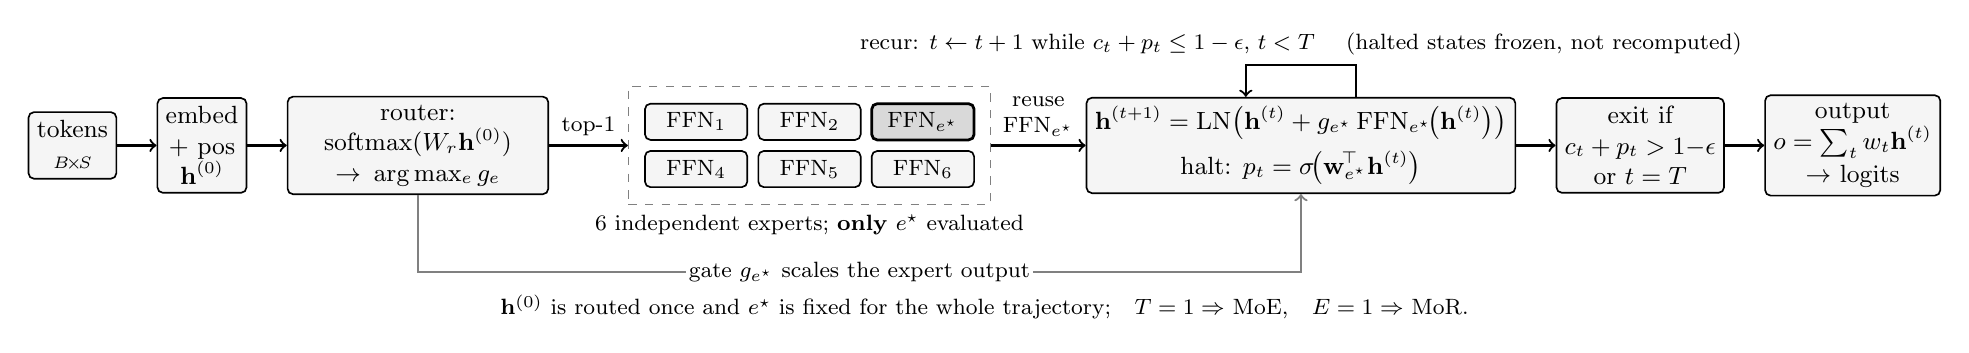
\begin{tikzpicture}[font=\small]
  \tikzset{
    box/.style = {draw, rounded corners=2pt, align=center, inner sep=3pt,
                  minimum height=7mm, line width=0.6pt},
    st/.style  = {box, fill=black!4},
    ex/.style  = {box, fill=black!4, minimum width=13mm, minimum height=4.6mm,
                  inner sep=1.5pt, font=\footnotesize},
    sel/.style = {box, fill=black!15, minimum width=13mm, minimum height=4.6mm,
                  inner sep=1.5pt, font=\footnotesize, line width=1.0pt},
    nb/.style  = {font=\footnotesize, align=center, inner sep=2pt},
    ar/.style  = {->, thick}
  }

  % ---- main row (each node is placed relative to its left neighbour) ----
  \node[st] (tok) at (0,0) {tokens\\ $\scriptstyle B\!\times\!S$};
  \node[st, anchor=west] (emb) at ([xshift=5mm]tok.east) {embed\\ $+$ pos\\ $\mathbf{h}^{(0)}$};
  \node[st, anchor=west, text width=31mm] (rtr) at ([xshift=5mm]emb.east)
       {router:\\ $\mathrm{softmax}(W_r\mathbf{h}^{(0)})$\\ $\to \arg\max_e g_e$};

  % expert bank: 2 x 3 grid, dashed frame
  \node[draw, dashed, gray, anchor=west, minimum width=46mm, minimum height=15mm]
       (bank) at ([xshift=10mm]rtr.east) {};
  \node[ex]  (e1) at ([xshift=-14.4mm,yshift= 3mm]bank.center) {FFN$_{1}$};
  \node[ex]  (e2) at ([xshift=  0mm,  yshift= 3mm]bank.center) {FFN$_{2}$};
  \node[sel] (e3) at ([xshift= 14.4mm,yshift= 3mm]bank.center) {FFN$_{e^\star}$};
  \node[ex]  (e4) at ([xshift=-14.4mm,yshift=-3mm]bank.center) {FFN$_{4}$};
  \node[ex]  (e5) at ([xshift=  0mm,  yshift=-3mm]bank.center) {FFN$_{5}$};
  \node[ex]  (e6) at ([xshift= 14.4mm,yshift=-3mm]bank.center) {FFN$_{6}$};
  \node[nb, anchor=north] at ([yshift=-0.5mm]bank.south)
       {6 independent experts; \textbf{only} $e^\star$ evaluated};

  % tied recursion block (Eq. 1 + Eq. 2)
  \node[st, anchor=west, minimum width=42mm] (rec) at ([xshift=12mm]bank.east)
       {$\mathbf{h}^{(t+1)}=\mathrm{LN}\!\left(
          \mathbf{h}^{(t)} + g_{e^\star}\,\mathrm{FFN}_{e^\star}\!\big(\mathbf{h}^{(t)}\big)
        \right)$\\[3pt]
        halt: $p_t=\sigma\!\big(\mathbf{w}_{e^\star}^{\!\top}\mathbf{h}^{(t)}\big)$};

  % exit decision (Eq. 3) and output
  \node[st, anchor=west] (exit) at ([xshift=5mm]rec.east)
       {exit if\\ $c_t+p_t>1{-}\epsilon$\\ or $t=T$};
  \node[st, anchor=west] (out) at ([xshift=5mm]exit.east)
       {output\\ $o=\sum_t w_t\mathbf{h}^{(t)}$\\[1pt] $\to$ logits};

  % ---- main-path arrows ----
  \draw[ar] (tok) -- (emb);
  \draw[ar] (emb) -- (rtr);
  \draw[ar] (rtr.east) -- (bank.west) node[midway, above=1pt, nb] {top-1};
  \draw[ar] (bank.east) -- (rec.west) node[midway, above=1pt, nb, align=center]
        {reuse\\ $\mathrm{FFN}_{e^\star}$};
  \draw[ar] (rec) -- (exit);
  \draw[ar] (exit) -- (out);

  % gate g_{e*} scales the expert output (router -> recursion block)
  \coordinate (gA) at ([yshift=-8.5mm]rtr.south |- bank.south);
  \coordinate (gB) at (rec.south |- gA);
  \draw[ar, gray] (rtr.south) -- (gA) -- (gB) -- (rec.south);
  \path (gA) -- (gB) node[midway, nb, fill=white, inner sep=1pt] {gate $g_{e^\star}$ scales the expert output};

  % recursion self-loop
  \draw[ar] ([xshift=7mm]rec.north) -- ([xshift=7mm,yshift=4mm]rec.north)
        -- ([xshift=-7mm,yshift=4mm]rec.north) -- ([xshift=-7mm]rec.north);
  \node[nb, anchor=south] at ([yshift=4.5mm]rec.north)
       {recur: $t \leftarrow t+1$ while $c_t+p_t\le 1-\epsilon$, $t<T$
        \quad(halted states frozen, not recomputed)};

  % bottom note
  \node[nb, anchor=north] at ([yshift=-0.5mm]current bounding box.south)
       {$\mathbf{h}^{(0)}$ is routed once and $e^\star$ is fixed for the whole
        trajectory;\quad $T=1\Rightarrow$ MoE,\quad $E=1\Rightarrow$ MoR.};
\end{tikzpicture}}
\caption{The MoRE block, drawn in TikZ. A token is routed \emph{once} from its
post-embedding state to one of $E$ independent expert FFNs, and \emph{that
expert's} weights---never another's---are reused for an adaptive number of
recursion steps under ACT halting. Only the selected expert is evaluated, and
its output is scaled by the gate $g_{e^\star}$. Setting $T=1$ recovers MoE
exactly and setting $E=1$ recovers MoR; the input representation is bit-identical
in all three cases, and all three are configurations of one engine.}
\label{fig:architecture}
\end{figure}
